\documentclass[a4paper,11pt]{article}
\usepackage[left=2cm,text={17cm,24cm},top=3cm]{geometry}
\usepackage[czech]{babel}
\usepackage[T1]{fontenc}
\usepackage{times}
\usepackage{caption}
\usepackage{multirow}
\usepackage{multicol}
\usepackage[ruled,vlined]{algorithm2e}
\usepackage{graphicx}
\usepackage{pdflscape}


\begin{document}

    \begin{titlepage}
        \begin{center}
            \textsc{\Huge{Vysoké učení technické v Brně}} \\
            \vspace{0.5 em}
            \textsc{\huge{Fakulta informačních technologií}} \\
            \vspace{\stretch{0.382}}
            \LARGE{Typografie a publikování\,--\,3. projekt} \\
            \Huge{Tabulky a obrázky}
            \vspace{\stretch{0.618}}
        \end{center}
        \Large{\today \hfill Jan Černoch}
    \end{titlepage}

\section{Úvodní strana}
Název práce umístěte do zlatého řezu a nezapomeňte uvést \textit{dnešní} (today) datum a vaše jméno a přijímení.

\section{Tabulky}
Pro sázení tabulek můžeme použít buď prostředí \verb|tabbing| nebo prostředí \verb|tabular|.

\subsection{Prostředí \texttt{tabbing}}

Při použití \verb|tabbing| vypadá tabulka následovně:
\begin{tabbing}
    \textbf{Ovoce} \hspace{1,5cm} \= \textbf{Množství} \hspace{0,3cm} \= \textbf{Jednotka} \hspace{0,3cm} \= \textbf{Cena za jedn.} \hspace{0,5cm} \= \textbf{Cena celková} \= \\
    Jablka\>        3\>     kg\>    25,90 Kč\>      77,70 Kč\\
    Hrušky\>        2,5\>   kg\>    27,40 Kč\>      68,50 Kč\\
    Vodní melouny\> 1\>     kus\>   36,\,-- Kč\>    36,\,-- Kč\\
\end{tabbing}
Toto prostředí se dá také použít pro sázení algoritmů, ovšem vhodnější je použít prostředí \verb|algorithm| nebo \verb|algorithm2e| (viz sekce 3).

\subsection{Prostředí \texttt{tabular}}
Další možností, jak vytvořit tabulku, je použít prostředí \verb|tabular|. Tabulky pak budou vypadat takto\footnote{Kdyby byl problem s \texttt{cline}, zkuste se podívat třeba sem: http://www.abclinuxu.cz/tex/poradna/show/325037.}:
\\
\begin{table}[h] \catcode`\-=12
    \centering
    \begin{tabular}{| l | c | c |} \hline
        & \multicolumn{2}{c |}{\textbf{Cena}} \\
        \cline{2-3}
        \textbf{Měna} & \textbf{Nákup} & \textbf{Prodej} \\
        \hline
        EUR & 24,45 & 25,93 \\
        GBP & 29,56 & 29,83 \\
        USD & 21,09 & 22,12 \\
        \hline
        \end{tabular}
        \caption{Tabulka kurzů k dnešnímu dni}
        \label{Kurzy}
\end{table}

\begin{table}[ht] \catcode`\-=12
    \centering
    \begin{tabular}{|c|c|} \hline
        $A$ & $\neg A$ \\ \hline
        \textbf{P} & N \\ \hline
        \textbf{O} & O \\ \hline
        \textbf{X} & X \\ \hline
        \textbf{N} & P \\ \hline
    \end{tabular}
    \begin{tabular}{|c|c|c|c|c|c|} \hline
        \multicolumn{2}{|c|}{\multirow{2}{*}{$A \wedge B$}} & \multicolumn{4}{c|}{B} \\ \cline{3-6}
        \multicolumn{2}{|c|}{} & \textbf{P} & \textbf{O} & \textbf{X} & \textbf{N} \\ \hline
        \multirow{4}{*}{A}  & \textbf{P} & P & O & X & N \\ \cline{2-6}
                            & \textbf{O} & O & O & N & N \\ \cline{2-6}
                            & \textbf{X} & X & N & X & N \\ \cline{2-6}
                            & \textbf{N} & N & N & N & N \\ \hline
    \end{tabular}
    \begin{tabular}{|c|c|c|c|c|c|} \hline
        \multicolumn{2}{|c|}{\multirow{2}{*}{$A \vee B$}} & \multicolumn{4}{c|}{B} \\ \cline{3-6}
        \multicolumn{2}{|c|}{} & \textbf{P} & \textbf{O} & \textbf{X} & \textbf{N} \\ \hline
        \multirow{4}{*}{A}  & \textbf{P} & P & P & P & P \\ \cline{2-6}
                            & \textbf{O} & P & O & P & O \\ \cline{2-6}
                            & \textbf{X} & P & P & X & X \\ \cline{2-6}
                            & \textbf{N} & P & O & X & N \\ \hline
    \end{tabular}
    \begin{tabular}{|c|c|c|c|c|c|} \hline
        \multicolumn{2}{|c|}{\multirow{2}{*}{$A \rightarrow B$}} & \multicolumn{4}{c|}{B} \\ \cline{3-6}
        \multicolumn{2}{|c|}{} & \textbf{P} & \textbf{O} & \textbf{X} & \textbf{N} \\ \hline
        \multirow{4}{*}{A}  & \textbf{P} & P & O & X & N \\ \cline{2-6}
                            & \textbf{O} & P & O & P & O \\ \cline{2-6}
                            & \textbf{X} & P & P & X & X \\ \cline{2-6}
                            & \textbf{N} & P & P & P & P \\ \hline
    \end{tabular}
    \caption{Protože Kleeneho trojhodnotová logina už je \uv{zastaralá}, uvádíme se zde příklad čtyřhodnotové logiky}
    \label{tab:my_label}
\end{table}
\clearpage


\section{Algoritmy}
Pokud budeme chtít vysázet algoritmus, můžeme použít prostředí \verb|algorithm|\footnote{http://ftp.cstug.cz/pub/tex/CTAN/macros/latex/contrib/algorithms/algorithms.pdf.} nebo \texttt{algorithm2e}\footnote{http://ftp.cstug.cz/pub/tex/CTAN/macros/latex/contrib/algorithm2e/doc/algorithm2e.pdf.}. Příklad použití prostředí \verb|algorithm2e| viz Algoritmus 1.

\begin{algorithm}
    \caption{{\textsc{FastSLAM}}}
    \textbf{Input:} $(X_{t-1}, u_t,z_t)$ \\
    \textbf{Output:} $X_t$ \\
    \SetAlgoLined
    \SetNlSty{}{}{:}
    \qquad\nlset{1}{$\overline{X_t} = X_t = 0$} \\
    \qquad\nlset{2}{\textbf{for} $k = 1$ to $M$ \textbf{do}} \\
    \qquad\nlset{3}\qquad{$x_{t}^{[k]} =$ \textit{sample\_motion\_model}$(u_t, x_{t-1}^{[k]})$} \\
    \qquad\nlset{4}\qquad$\omega_{t}^{[k]} =$ \textit{measurement\_model}$(z_t, x_t^{[k]}, m_{t-1})$ \\
    \qquad\nlset{5}\qquad $m_t^{[k]} =$ \textit{updated\_occupancy\_grid}$(z_t, x_t^{[k]}, m_{t-1}^{[k]})$ \\
    \qquad\nlset{6}\qquad $\overline{X_t} = \overline{X_t} + \langle x_x^{[m]}, \omega_t^{[m]} \rangle$ \\
    \qquad\nlset{7} \textbf{end for} \\
    \qquad\nlset{8} \textbf{for} $k = 1$ to $M$ \textbf{do} \\
    \qquad\nlset{9}\qquad draw $i$ with probability $\approx \omega_t^{[i]}$ \\
    \qquad\nlset{10}\qquad add $\langle x_x^{[k]}, m_t^{[k]} \rangle$ to $X_t$ \\
    \qquad\nlset{11} \textbf{end for} \\
    \qquad\nlset{12} \textbf{return} $X_t$
\end{algorithm}

\section{Obrázky}
Do našich článků můžeme samozřejmě vkládat obrázky. Pokud je obrázkem fotografie, můžeme klidně použít bitmapový soubor. Pokud by to ale mělo být nějaké schéma nebo něco podobného, je dobrým zvykem takovýto obrázek vytvořit vektorově.

\begin{figure}[ht]
    \centering
    \scalebox{0.4}{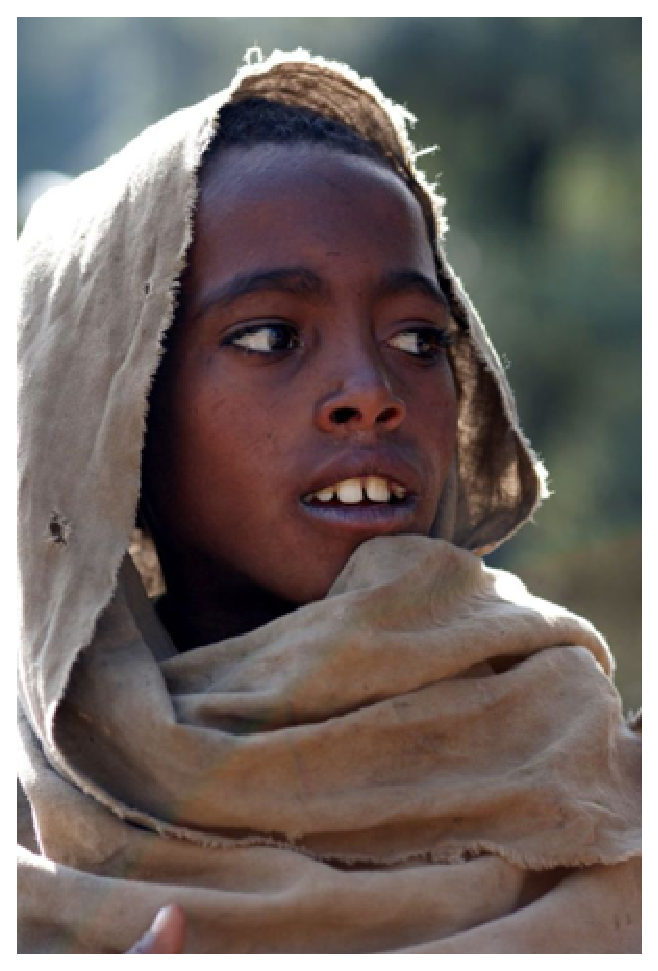
\includegraphics{etiopan.eps}}
    \scalebox{0.4}{\reflectbox{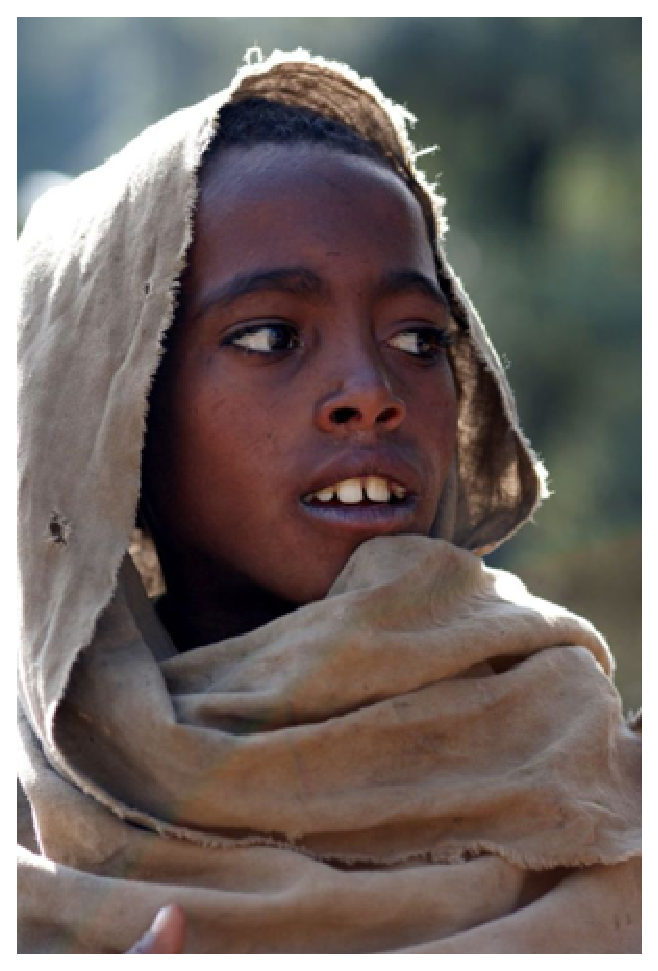
\includegraphics{etiopan.eps}}}
    \caption{Malý Etiopánek a jeho bratříček}
\end{figure}

\clearpage

Rozdíl mezi vektorovým\,\dots
\begin{figure}[ht]
    \centering
    \scalebox{0.4}{
\includegraphics{oniisan.eps}}
    \caption{Vektorový obrázek}
\end{figure}

\dots a bitmapovým obrázkem
\begin{figure} [ht]
    \centering
    \scalebox{0.6}{
\includegraphics{oniisan2.eps}}
    \caption{Bitmapový obrázek}
\end{figure} \\
se projeví například při zvětšení.

Odkazy (nejen ty) na obrázky 1, 2 a 3, na tabulky 1 a 2 a také na algoritmus 1 jsou udělány pomocí křížových odkazů. Pak je ovšem potřeba zdrojový soubor přeložit dvakrát. 

Vektorové obrázky lze vytvořit i přímo v \LaTeX u, například pomocí prostředí \verb|picture|.

\clearpage

\begin{landscape}
    \begin{figure}
        \setlength{\unitlength}{1.5mm}
        \centering
        \begin{picture}(120,60)

              % House base
              \put(10,10){\line(1,0){90}}
              \put(10,10){\line(0,1){40}}
              \put(100,10){\line(0,1){40}}
              \put(10,50){\line(1,0){90}}
            
              % Roof
              \put(10,50){\line(1,0){90}}
              \put(10,50){\line(2,1){20}}
              \put(100,50){\line(-2,1){20}}
              \put(30,60){\line(1,0){50}}
            
              % Chimney
              \put(60,60){\line(0,1){10}}
              \put(65,60){\line(0,1){10}}
              \put(60,70){\line(1,0){5}}
            
              % Left entrance block
              \put(10,10){\line(-1,0){10}}
              \put(0,10){\line(0,1){30}}
              \put(0,40){\line(1,0){10}}
            
              % Door
              \put(3,10){\line(0,1){15}}
              \put(8,10){\line(0,1){15}}
              \put(3,25){\line(1,0){5}}
            
              % Balcony
              \put(35,30){\line(1,0){30}}
              \put(35,25){\line(1,0){30}}
              \put(35,25){\line(0,1){5}}
              \put(65,25){\line(0,1){5}}
            
              % Balcony railing
              \multiput(37,25)(3,0){9}{\line(0,1){5}}
            
              % Upper left window
              \put(42,35){\line(1,0){16}}
              \put(42,35){\line(0,1){10}}
              \put(58,35){\line(0,1){10}}
              \put(42,45){\line(1,0){16}}
              \put(50,35){\line(0,1){10}}
            
              % Upper right window
              \put(72,35){\line(1,0){16}}
              \put(72,35){\line(0,1){10}}
              \put(88,35){\line(0,1){10}}
              \put(72,45){\line(1,0){16}}
              \put(80,35){\line(0,1){10}}
            
              % Lower left window
              \put(40,15){\line(1,0){18}}
              \put(40,15){\line(0,1){10}}
              \put(58,15){\line(0,1){10}}
              \put(40,25){\line(1,0){18}}
              \put(49,15){\line(0,1){10}}
            
              % Lower right window
              \put(72,15){\line(1,0){18}}
              \put(72,15){\line(0,1){10}}
              \put(90,15){\line(0,1){10}}
              \put(72,25){\line(1,0){18}}
              \put(81,15){\line(0,1){10}}
            
              % Sun
              \put(95,70){\circle{8}}
                
              % rays
              \put(95,74){\line(0,1){4}}
              \put(95,66){\line(0,-1){4}}
              \put(99,70){\line(1,0){4}}
              \put(91,70){\line(-1,0){4}}
                
              \put(98,73){\line(1,1){3}}
              \put(92,73){\line(-1,1){3}}
              \put(98,67){\line(1,-1){3}}
              \put(92,67){\line(-1,-1){3}}

              % Ground line
              \linethickness{1.8pt}
              \put(0,10){\line(1,0){100}}
              
        \end{picture}
        \caption{Schematické znázornění mého domova vytvořené v prostředí picture}
    \end{figure}
\end{landscape}

\end{document}
